\namedchapter[Adam Zieliński]{Rys historyczny}
Słowo ,,robot" wywodzi się z języka czeskiego, gdzie oznacza ciężką pracę. 
Według słownika języka polskiego słowo to oznacza urządzenie zastępujące człowieka przy wykonywaniu niektórych czynności\cite{SJP}. Po raz pierwszy, w tym kontekście, zostało ono użyte w 1920 r. przez czeskiego pisarza Karela \newtie{C}apka w komedii R.U.R.(Rossum Universal Robots)\cite{Czech}. Precyzyjną definicję tego słowa przedstawiła w 1979 roku grupa \textit{Robotics Industries Association} określając robota jako: ,,Programowalny, wielofunkcyjny manipulator zaprojektowany do przenoszenia materiałów, części, narzędzi lub specjalizowanych urządzeń poprzez różne programowalne ruchy, w celu realizacji różnorodnych zadań."\cite{def_robota}.
Temat robotyki był bardzo często i szeroko poruszany przez pisarzy fantastyki naukowej, którzy w swoich dziełach wykorzystywali motyw buntu maszyn przeciwko ludzkości. Efektem tego było pojawienie się trendu filozoficznego mówiącego o etyce robotów. Jednym z twórców tego nurtu, Isaac Asimow, zaproponował kilka reguł, którymi powinna kierować się każda inteligentna maszyna\cite{prawa_robota}:
\begin{enumerate}
\item Robot nie może skrzywdzić człowieka, ani przez zaniechanie działania dopuścić, aby człowiek doznał krzywdy.
\item Robot musi być posłuszny rozkazom człowieka, chyba że stoją one w sprzeczności z Pierwszym Prawem.
\item Robot musi chronić sam siebie, jeśli tylko nie stoi to w sprzeczności z Pierwszym lub Drugim Prawem.
\end{enumerate}
Mówi się, że robotyka jest owocem wszystkich dotychczasowych osiągnięć ludzkości w każdej dziedzinie. Łączy w sobie przede wszystkim elementy: mechaniki, automatyki, elektroniki, sensoryki oraz cybernetyki.
Jej poszczególne elementy były rozwijane na przestrzeni setek a nawet tysięcy lat. Pierwsze wzmianki historyczne dotyczące budowy robotów sięgają około 350 roku p.n.e. i dotyczą greckiego matematyka Archtasa z Tarentu, który rzekomo zbudował ptaka napędzanego sprężonym powietrzem oraz potrafiącego latać. Niestety  zweryfikowanie tej wiadomości jest bardzo skomplikowane i nie daje jednoznacznej odpowiedzi. Wskazuje ona jednak na zainteresowanie ludzkości budową maszyn-robotów, które pierwotnie miały naśladować naturę. Za początek rozwoju robotyki uważa się przełom XV oraz XVI wieku, w którym za sprawą wielkiego wynalazcy - Leonadra da Vinci powstało wiele interesujących konstrukcji. Jego projekty niejednokrotnie znacznie wykraczały poza czasy, w których żył. W swoich badaniach pozostawał wierny aforyzmowi ,,Mądrość jest
córką doświadczenia" - w związku z czym zaprojektowane przez niego konstrukcje nie opierały się na dotychczasowych teoretycznych osiągnięciach ówczesnej Europy a na własnych badaniach, pomiarach oraz próbach\cite{da_vinci}.  Na ilustracji \ref{czolg_leon} przedstawiony został szkic przedstawiający jedną z wymyślonych przez Leonarda da Vinci maszyn wojennych - przodek współczesnego czołgu, który miał miotać kamieniami w wroga oraz być napędzany siłą ludzkich mięśni.

  \begin{figure}[H]
    \begin{center}
      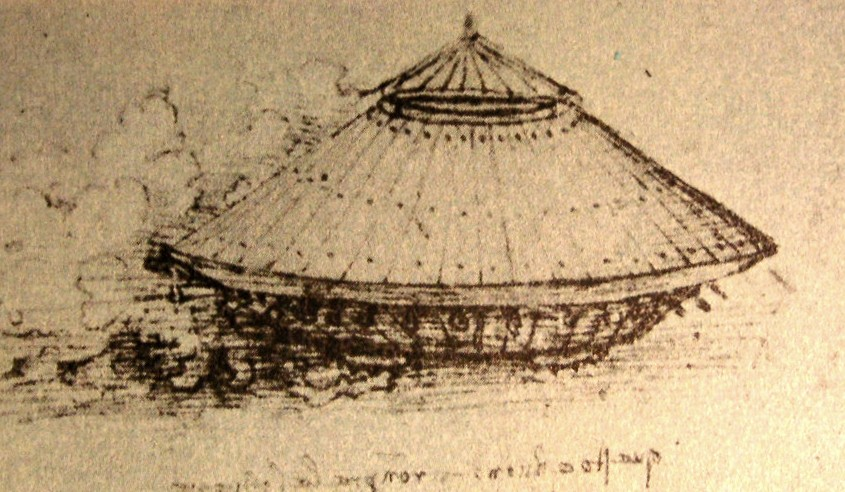
\includegraphics[scale=0.25]{imgs/Leonardo_tank.jpg}
 	\caption[Czołg Leonarda da Vinci]{\small{Szkic Leonarda da Vinci przedstawiający jego koncepcję czołgu.}\footnotemark}
	\label{czolg_leon}
    \end{center}
  \end{figure}
  \footnotetext{\emph{Czołg Leonarda da Vinci}, http://italoteka.blogspot.com,  (data dostępu 21.04.2015r.)}
Wiek XX niesie za sobą bardzo gwałtowny rozwój robotyki, który rozpoczął się w momencie skonstruowania w latach 40-tych pierwszego komputera. Ich rozwój był dodatkowo spotęgowany poprzez wybuch II wojny światowej i potrzebę łamania szyfrów dyplomatycznych.
W latach 50-tych wynaleziony został tranzystor, który aktualnie jest podstawowym elementem każdego urządzenia. Pozwolił on w znacznej mierze na zmniejszenie gabarytów komputerów (jednostek obliczeniowych), zmniejszenie zapotrzebowania na energię oraz wzrost mocy obliczeniowej co pozwoliło na konstrukcję autonomicznych robotów mobilnych.
Robotami mobilnymi nazywamy pojazdy, mogące zmieniać swoje położenie w przestrzeni. Dotyczy to nie tylko pojazdów jezdnych, ale także kroczących czy latających. 
W 1956 r. ukończona została budowa elektrycznej wiewiórki\cite{robot_squee} (rysunek \ref{squee}), która posiadała dwa ,,zmysły": wzroku - zrealizowanego przy wykorzystaniu dwóch lamp fotoelektronowych oraz dotyku - dwóch krańcówek.  Napęd został zbudowany w oparciu o silniki elektryczne. Zwierzak, gdy zobaczył żołędzia (w tym przypadku jasno oświetlony punkt) kierował się w jego stronę, podnosił owoc przy pomocy ,,szufli" a następnie kierował się ,,do gniazda" - czyli miejsca, gdzie znajdowało się pulsacyjne źródło światła. Mimo ,iż realizowane zadanie jest bardzo proste to możemy mówić tutaj o pewnego rodzaju inteligencji ponieważ wiewiórka wykonywała pewną sekwencję ruchową bez interwencji człowieka ale w zależności od tego, co działo się w jej otoczeniu.

  \begin{figure}[H]
    \begin{center}
      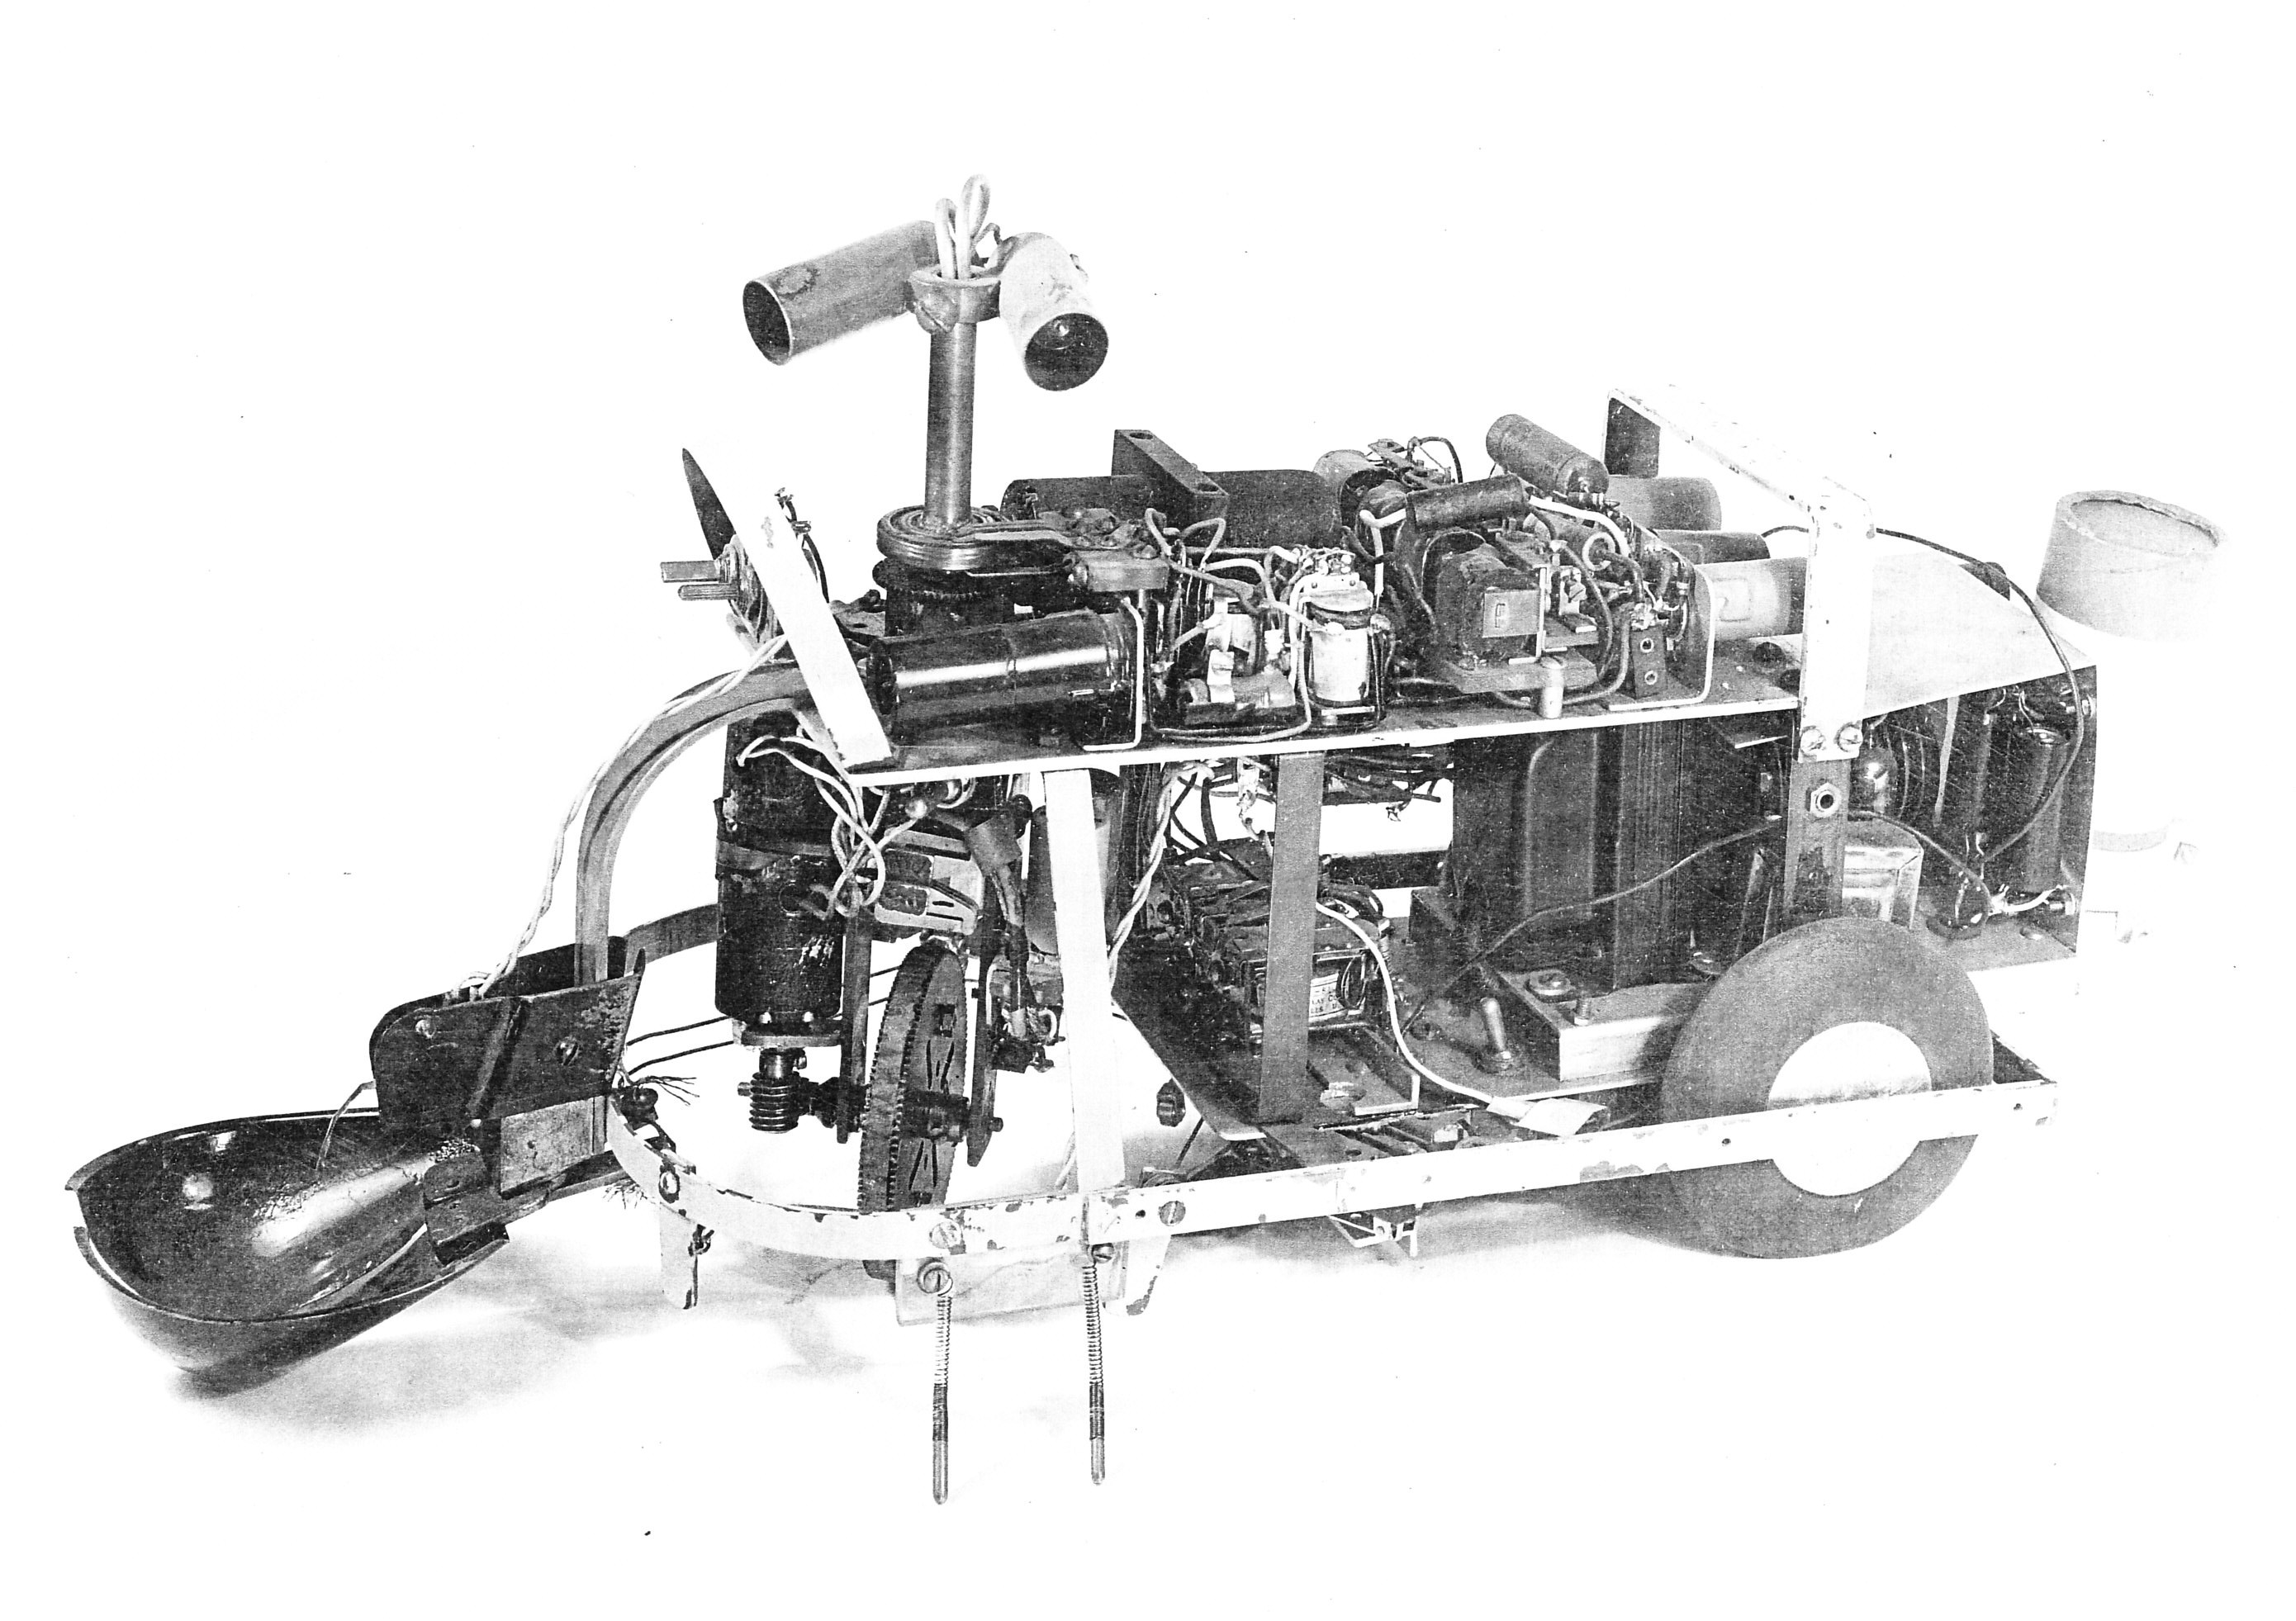
\includegraphics[scale=0.35]{imgs/Squee.jpg}
 \caption[Robot \textit{Squee}]{\small{Robot Squee zbudowany prze Jacka Koffa w 1959r.}\footnotemark}
        \label{squee}
    \end{center}
  \end{figure}
  \footnotetext{\emph{Robot Squee}, http://cyberneticzoo.com/,  (data dostępu 21.09.2015r.)}

Kolejne lata niosą za sobą coraz większą miniaturyzację wszelkich podzespołów elektronicznych. Nie tylko zamykane są one w coraz mniejszych obudowach (pierwszy układ scalony - Jack St. Clair Kilby w 1958 r.) ale także charakteryzują się coraz wyższą sprawnością. Doprowadza to do tego, że pojazdy mobilne stają się obiektem zainteresowania służb specjalnych. W ten sposób w 1984 r. powstaje Prowler (rysunek \ref{state}) - pierwszy zdalnie sterowany robot o przeznaczeniu militarnym. Platforma ta mogła pełnić różne funkcje: od roli wsparcia - wyposażona w karabiny maszynowe, po funkcje rozpoznawcze - wyposażona w kamery.

  \begin{figure}[H]
    \begin{center}
      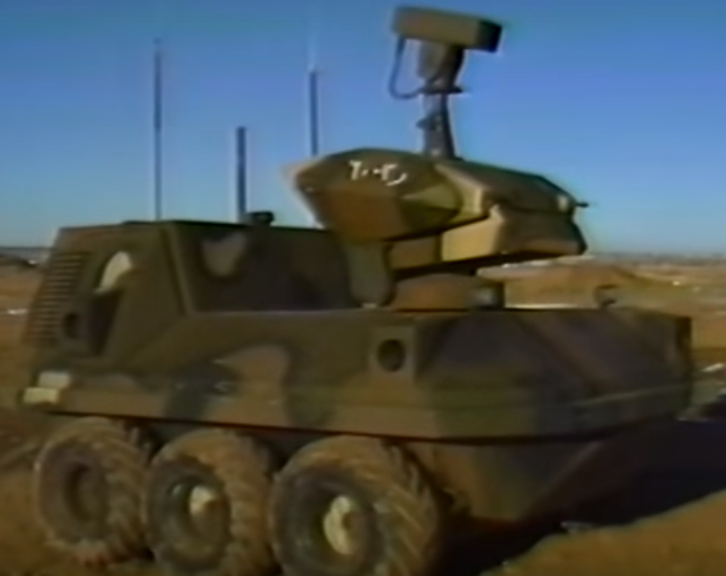
\includegraphics[scale=0.4]{imgs/state.png}
 \caption[Pojaz wojskowy \textit{Prowler}]{\small{Wojskowy robot mobilny Prowler .}\footnotemark}
        \label{state}
    \end{center}
  \end{figure}
  \footnotetext{\emph{Robot Defense Systems Prowler 1985}, https://youtube.com/,  (data dostępu 22.09.2015r.)}

Aktualnie najbardziej zaawansowanymi robotami mobilnymi są pojazdy wykorzystywane przez agencje kosmiczne do eksploracji kosmosu. Ich konstrukcja jest efektem bardzo rygorystycznych założeń jakie są im stawiane, tzn.: możliwie jak najmniejsze rozmiary, waga, wysoka mobilność oraz niezawodność, możliwość pracy w ciężkich, nieznanych warunkach środowiskowych. Na dodatek muszą one być zdolne do prowadzenia badań oraz zbierania próbek. Przykładem tej klasy robota może być marsjański łazik Curiosity Rover (rysunek \ref{lazik}).

  \begin{figure}[H]
    \begin{center}
      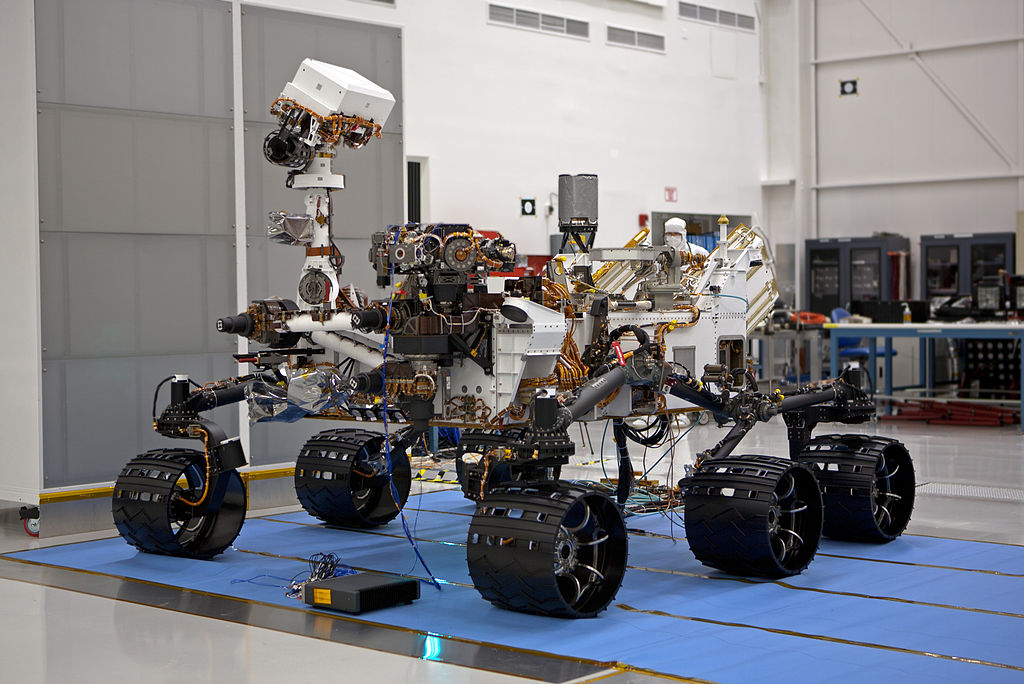
\includegraphics[scale=0.8]{imgs/curiosity.png}
 \caption[Łazik marsjański \textit{Curiosity}]{\small{Łazik marsjański Curiosity.}\footnotemark}
        \label{lazik}
    \end{center}
  \end{figure}
  \footnotetext{\emph{\textit{Curiosity}}, http://i.space.com/,  (data dostępu 22.09.2015r.)}
